\documentclass[11pt]{article}
\usepackage[table]{xcolor} %colour cells in tables
\usepackage[bottom]{footmisc} % footnotes at the bottom
%\usepackage{indentfirst}
\usepackage{pdfpages}
\renewcommand{\baselinestretch}{1.5} 
%% Language and font encodings
\usepackage[T1]{fontenc}
\usepackage{array}
%% Sets page size and margins

%\linespread{1.3} % spacing between lines - 1.3 for space and half
\usepackage{fancyhdr}
\usepackage[top=2.6cm, bottom=4.1cm, right=2cm, left=2cm, headsep=1.1cm]{geometry}
\usepackage{listings}

\setlength{\headheight}{52pt}
\usepackage{fontspec}
\usepackage{multicol}
%centered text
\newenvironment{tightcenter}{%
  \setlength\topsep{0pt}
  \setlength\parskip{0pt}
  \begin{center}
}{%
  \end{center}
}

\lstset{literate=
  {á}{{\'a}}1 {é}{{\'e}}1 {í}{{\'i}}1 {ó}{{\'o}}1 {ú}{{\'u}}1
  {Á}{{\'A}}1 {É}{{\'E}}1 {Í}{{\'I}}1 {Ó}{{\'O}}1 {Ú}{{\'U}}1
  {à}{{\`a}}1 {è}{{\`e}}1 {ì}{{\`i}}1 {ò}{{\`o}}1 {ù}{{\`u}}1
  {À}{{\`A}}1 {È}{{\'E}}1 {Ì}{{\`I}}1 {Ò}{{\`O}}1 {Ù}{{\`U}}1
  {ä}{{\"a}}1 {ë}{{\"e}}1 {ï}{{\"i}}1 {ö}{{\"o}}1 {ü}{{\"u}}1
  {Ä}{{\"A}}1 {Ë}{{\"E}}1 {Ï}{{\"I}}1 {Ö}{{\"O}}1 {Ü}{{\"U}}1
  {â}{{\^a}}1 {ê}{{\^e}}1 {î}{{\^i}}1 {ô}{{\^o}}1 {û}{{\^u}}1
  {Â}{{\^A}}1 {Ê}{{\^E}}1 {Î}{{\^I}}1 {Ô}{{\^O}}1 {Û}{{\^U}}1
  {œ}{{\oe}}1 {Œ}{{\OE}}1 {æ}{{\ae}}1 {Æ}{{\AE}}1 {ß}{{\ss}}1
  {ű}{{\H{u}}}1 {Ű}{{\H{U}}}1 {ő}{{\H{o}}}1 {Ő}{{\H{O}}}1
  {ç}{{\c c}}1 {Ç}{{\c C}}1 {ø}{{\o}}1 {å}{{\r a}}1 {Å}{{\r A}}1
  {€}{{\euro}}1 {£}{{\pounds}}1 {«}{{\guillemotleft}}1
  {»}{{\guillemotright}}1 {ñ}{{\~n}}1 {Ñ}{{\~N}}1 {¿}{{?`}}1
}
\usepackage{listings}
\lstdefinestyle{customc}{
  belowcaptionskip=1\baselineskip,
  breaklines=true,
  frame=L,
  xleftmargin=\parindent,
  language=Matlab,
  showstringspaces=false,
   numbers=left,%
    numberstyle={\tiny \color{black}},% size of the numbers
    numbersep=9pt,
  basicstyle=\footnotesize\ttfamily,
  keywordstyle=\bfseries\color{green!40!black},
  commentstyle=\itshape\color{purple!40!black},
  identifierstyle=\color{blue},
  stringstyle=\color{orange},
}
\lstset{style=customc}
\usepackage{matlab-prettifier}

\usepackage{textcomp}
\usepackage{graphicx}        %imagens
\usepackage{siunitx}
\usepackage{units}
\usepackage{float}
\usepackage{amssymb}
\usepackage{gensymb}
\usepackage{mathtools}
\usepackage{amsmath}
\usepackage{bm}
\usepackage{commath}
\usepackage[all]{nowidow}           %para evitar frases orfãs
\usepackage{float} 
\usepackage{hyperref}
\def\UrlBreaks{\do\/\do-}
% \usepackage[hyphenbreaks]{breakurl}
% \usepackage[hyphens]{url}
\usepackage[nottoc,notlof,notlot]{tocbibind} 
\setcounter{tocdepth}{3} %don't have subsubsubsections on table of contents
\usepackage{ragged2e}
\usepackage{refcount}
%\usepackage[noadjust]{cite}
\usepackage{tocloft}

\usepackage[titletoc,title]{appendix}

\usepackage[justification=centering]{caption}
\usepackage{subcaption}

\usepackage[numbers,sort&compress]{natbib}

\usepackage{tabularx}  % split table lines
    \newcolumntype{L}{>{\centering\arraybackslash}X}
    \renewcommand\tabularxcolumn[1]{m{#1}} 
    
    \newcolumntype{R}{>{\RaggedRight\arraybackslash}X}
    \renewcommand\tabularxcolumn[1]{m{#1}} %centering vertically
    
\usepackage{booktabs} %toprule and midrule
\usepackage{pgfplots}

%\usepackage{slashbox} %to divide cells in half with a backslash
\usepackage{pifont}

\let\savedegree\degree
\let\degree\relax
\usepackage{mathabx}
\let\degree\savedegree
\usepackage{wasysym}

\usepackage{relsize} %big math symbols with \mathlarer{...}

\pgfplotsset{compat=1.14}

\usepackage{multirow}   %multirow for tables

%%%%%%%%%%%%%%%%% header and footer %%%%%%%%%%%%%%%%%%%%%
\lhead{
\includegraphics[scale=0.12]{TU-delft.png}}
\rhead{{Space Embedded Systems}}
\lfoot{Final Assignment -- Solar Panel Drive Mechanism}    %{Assignment}
\cfoot{}
\rfoot{\thepage}
\renewcommand{\headrulewidth}{0.3pt}
\renewcommand{\footrulewidth}{0.3pt}
%%%%%%%%%%%%%%%%% header and footer %%%%%%%%%%%%%%%%%%%%%
%\renewcommand{\thesubsection}{\thesection.\alph{subsection}}
\begin{document}

%%%%%%%%%%%%%%%%%%%%%%%% Cover %%%%%%%%%%%%%%%%%%%%%%%%%%%
\begin{titlepage}
\newcommand{\HRule}{\rule{\linewidth}{0.5mm}} % Defines a new command for the horizontal lines, change thickness here

\center 
\setlength{\headheight}{15pt}

\includegraphics[scale=0.45]{TU-delft.png}\\[1.5cm] 

\textsc{\LARGE Delft University of Technology}\\[2cm]
\textsc{\Large Space Embedded Systems\\ AE4S20 }\\[1cm] 

\HRule \\[0.2cm]
{\huge \bfseries Solar Panel Drive Mechanism\\[0.4cm]} % Title of your document
\HRule \\[0.1cm]
\vfill
\begin{table}[H]
    \centering
    \begin{tabular}{cc}
 Maxi Mira Gallbrecht & 4757289 \\
 Tiago Sousa Costa &  4832507
    \end{tabular}
\end{table}
\end{titlepage}
\setlength{\headheight}{52pt}
\pagebreak
%%%%%%%%%%%%%%%%%%%%%%%% Cover %%%%%%%%%%%%%%%%%%%%%%%%%%%

	\setcounter{page}{1}
	\pagenumbering{roman}
	\pagebreak
	\tableofcontents
	\cleardoublepage
	\pagebreak
	%\setcounter{page}{1}
	\pagenumbering{arabic}
	\pagestyle{fancy}


\section{Introduction}



\pagebreak
\section{Solar panel drive mechanism project}

iterative design process



\subsection{Subsystem requirements}


WOrking here aijsfpsuanfpawuinfpaiuenrfpiuaenwfpiuns<dçjfn<sçkjn

\begin{itemize}
    \item The subsystem shall be able to receive a command to set the solar panel at a certain angle.
    \item The subsystem shall implement the commands in a safe way.
    \item The subsystem shall give feedback. 
    \item The subsystem shall be failure tolerant to all of its components.
\end{itemize}
\pagebreak
\section{Mechatronics}
\label{sec:mechatronics}
This section specifies the components used for the solar panel drive mechanism. The implementation of hardware redundancy is considered during the design phase, since the system's fault tolerance is a driving aspect of this project. This redundancy is represented in the choice and quantity of specific components. Table \ref{tab:component_list} displays all the components, their quantities and corresponding details.

\subsection{Microcontroller}
This system uses an Arduino Mega 2560 microcontroller. Arduino offers not only boards containing the processor, memory, I/Os, and power system in a compact interface but also allows for easy software integration. To fulfil the requirement of fault tolerance, this system has a second microcontroller of the same kind in a watchdog configuration. Once the master microcontroller fails to reset the watchdog's timer, the second (slave) microcontroller takes over, in case the latter cannot reset the master board. This configuration uses an Arduino Mega 2560 instead of the Arduino Uno, due to the increased amount of pins available, which are required for the system to function properly, regarding the fault tolerance.

\subsection{Rotation mechanism}
To move the solar panel into the assigned angular position a motor is needed. For this project, an uni-polar stepper motor is used as the system's actuator. The idea is that the motor drives an axis on which the solar panel sits,  which is then rotated into the defined position. The motor rotates in fixed angular increments, instead of moving continuously, which makes stepper motors very precise and suitable for the application in a solar panel drive mechanism. Another advantage of the stepper motor is its capacity to hold torque also when it is not powered. The 28BYJ-48 stepper motor is used for the driving mechanism and integrated into the system setup through its the ULN2003 driver board. The other end of the rotation axis holds the potentiometer used to verify the angular position obtained by the stepper motor. Here, a concerning challenge is the reproducibility of the potentiometer feedback since its linear output has a standard tolerance of 20\% \cite{poti}. Figure \autoref{fig:components_rotation} depicts the stepper motor and its driver board, and the potentiometer.

\begin{figure}[H]
    \centering
    \begin{subfigure}[b]{0.3\textwidth}
       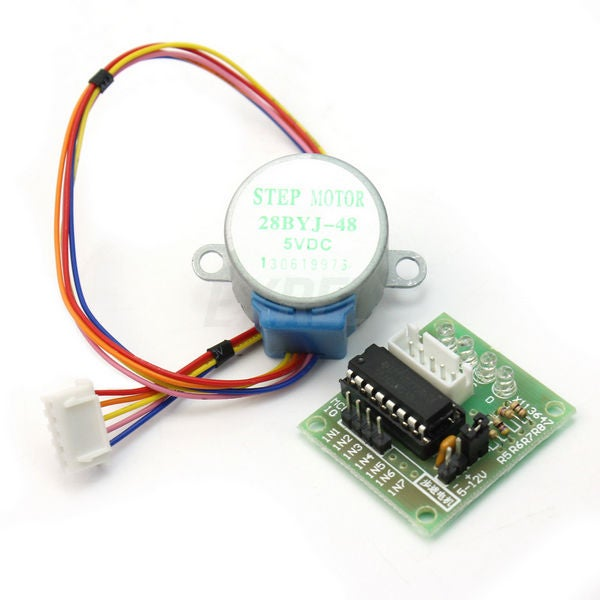
\includegraphics[width=\textwidth]{figures/steppermotor_board.jpg}
       \caption{28BYJ-48 stepper motor and ULN2003 driver board}
    \end{subfigure}
    \begin{subfigure}[b]{0.3\textwidth}
       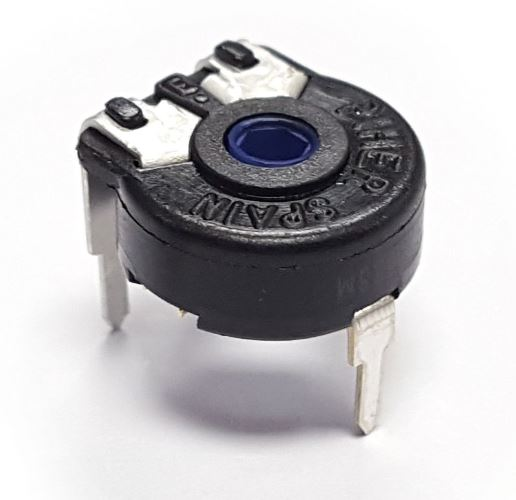
\includegraphics[width=\textwidth]{figures/pot.JPG}
       \caption{Piher PT10 potentiometer}
    \end{subfigure}
    \caption{Solar panel mounting structure}
    \label{fig:components_rotation}
\end{figure}{}


\subsection{Visual feedback}
Besides the serial monitor, the user receives visual feedback about the state of the system through a set of LEDs and an LCD screen. The former provides information regarding the operation status of the stepper motor. The latter shows the current angle of the solar panel and additional information about the system.

\subsection{Other components}
Two breadboards are part of the system setup accommodating the LEDs, LCD, and necessary jumper wires. The majority of wires are in male/male configuration, while male/female jumper wires connect the potentiometers and motor driver boards. Additionally, $\unit[220]{\Omega}$ resistors adjust the current flowing to the visual components.



\begin{table}[H]
    \centering
    \begin{tabular}{|l|r|c|}
        \hline
        Component   &  Quantity &  Details\\ \hline
        Microcontroller  & 2     & Arduino Mega 2560 plus USB cable\\
        Stepper motor & 2 & 28BYJ-48\\
        Stepper motor driver & 2 & ULN2003 driver board\\
        Potentiometer & 3 & Piher PT10 50K\\
        LCD screen & 1 & NDS1602A module\\
        LED (red \& green) & 4 &  --\\
        Resistor & 5 & 220 Ohm\\
        Breadboard & 2 & --\\
        Jumper wires & 30+ & male/male \& male/female \\
        \hline
    \end{tabular}
    \caption{List of components}
    \label{tab:component_list}
\end{table}{}
\pagebreak
\section{Failure analysis}
\label{sec:preliminary_analysis}
 The components listed in the previous section are subject to faults and possible failures. Thus, this preliminary failure analysis will guide the system design. To exclude possible system failures, this chapter considers different design solutions that address each of the components' weak points and probable faults that may occur during operation. 

\subsection{Stepper motor}
\begin{itemize}
    \item \textbf{Mechanical issues}\\
    The stepper motors are not very accurate and may occasionally drift or block. The design needs to address these issues with sufficient redundancy to avoid failure. This includes methods to reset the stepper motor and having a redundant stepper motor, for example.
    
    \item \textbf{No power}\\
    If the design fails to provide power to the stepper motor, the whole subsystem fails. A redundant stepper motor avoids this issue. 
    
    \item \textbf{Faulty feedback}\\
    The controller cannot rely solely on the stepper's feedback. The controller manages the stepper motor angle internally, i.e., the motor does not provide its real step, but the difference between the initial step and the current position. In the case the motor blocks, the controller might perceive that the motor is rotating. The design has to avoid this issue with other means of feedback for example (such as the potentiometers).
\end{itemize}



\subsection{Potentiometer}
\begin{itemize}
    \item \textbf{Mechanical issues}\\
    The potentiometers are going to be connected to the stepper motors, to emit feedback on the solar panel's angle. However, they can jam or block (alike the stepper motors) and this can prevent the proper functioning of the subsystem. Having redundant units helps with this issue.
    
    \item \textbf{Power loss}\\
    If the power connection fails, the potentiometer may provide wrong feedback. Similarly to the stepper motors, a redundant potentiometer is a possible solution.
    
    \item \textbf{Faulty feedback}\\
    The feedback from the potentiometer is not always reproducible (as addressed in \autoref{sec:mechatronics}). Having redundant units aids this issue, as the microcontroller can have more data to assess the state of the solar panel.
    
    
\end{itemize}

\subsection{Microcontroller}
\begin{itemize}
    \item  \textbf{No communication}\\ 
    If the communication is lost between the microcontroller and the actuators and/or sensors, the system is incapable of operating successfully. Additionally, if there is no communication with the sensors, it is not possible to verify the panel's angular position. Possible solutions are implementing a reset frequency to restart the operations and/or a second microcontroller.
    
    \item \textbf{No power}\\
    If the microcontroller has no power the operation of the solar panel drive mechanism fails. A second redundant microcontroller is a possible solution.   
    \item \textbf{Faulty hardware} \\
    The microcontroller is responsible for operating the complete system. Faulty operation of the Arduino Mega 2560 may lead to unpredictable issues. Since the microcontroller is an integrated and isolated unit, a solution for internal faults that can lead to the subsystem failure consists in implementing a second microcontroller.
\end{itemize}

\subsection{Other components}
\begin{itemize}
    \item \textbf{Computer issues}\\
    In case the connection to the computer is lost, the user cannot control to the system. The system's power supply originates via USB. Hence, if the power supply fails, the system is not operative. Recovering from this fault is highly complex and computer redundancy will not be considered.
    
    \item \textbf{Faulty cabling}\\
    The project set-up includes jumper cables and breadboards. Some connections may be loose or unsteady and can lead to communication or sensor feedback problems. Checking all the wiring before operating is therefore essential. 
    
    \item \textbf{LCD and LEDs failure}\\
    The LCD and the LEDs provide visual feedback on the state of the system. In case that both are not operational, there is no visual feedback. However, the system's main objective -- driving and controlling the solar panel -- is not obstructed. Hardware redundancy or the reset of the complete system are valid options to address the visual feedback of the system.
    
    \item \textbf{Solar panel model (including axis) mechanical failure}\\
    For this project the mock-up solar panel is attached to only one stepper motor and potentiometer via an axis. Mechanical failures of this scaled design are considered out of scope of this course.
\end{itemize}

 
 
\pagebreak
\section{System design}
This section depicts and elaborates on the solar panel drive's final hardware design. Design choices made within the circuit and mechanical design are explained. Further, the reasons for deployed redundancy, fault tolerance, and simplifications are given.

\subsection{Circuit design}
\autoref{fig:circuit_schematic} displays the complete circuit setup.
Since no single failure in any of the system's components shall compromise the operation of the solar panel drive, redundancy is applied for the microcontroller, actuator, and sensors. Thus, the setup integrated two Arduino Mega 2560. They function in a watchdog configuration, where the second microcontroller -- the slave -- is in hot standby and ready to take over. Both microcontrollers can command and receive feedback from the actuators and sensors. The Arduinos communicate with each other through their communication pins, shown in the orange and yellow wires from TX2/RX2 to RX3/TX3 in \autoref{fig:circuit_schematic}. 

This design includes two stepper motors. When stepper motor 1 is operative, stepper motor 2 is in stand by and ready to take over. The state of each of the stepper motors is indicated through four LEDs -- two red and two green. A constant green light indicates that the motor is in stand by and ready to receive commands, while a red light lets the user know that the respective motor is out of service and not operational. When a motor receives a command and rotates, both green and red LEDs are turned on. Likewise, the LCD prints which motor is active and its current angle. The LEDs and the LCD are solely connected to the master microcontroller. Although connecting the visual feedback components to the slave Arduino is simple, the experimental setup does not include this setup since there are limited jumper wires available. The code for the slave microcontroller, shown in appendix \ref{appendix:slave}, includes the functionality of the LEDs and LCD. The stepper motors connect to their respective driver boards and are powered through the 5V pin of the master Arduino. Redundancy is not applied for the powering of the motors. An external power source could be used, but for simplification reasons of the experimental setup, the Arduino is considered to be sufficient.

\begin{figure}[H]
    \centering
   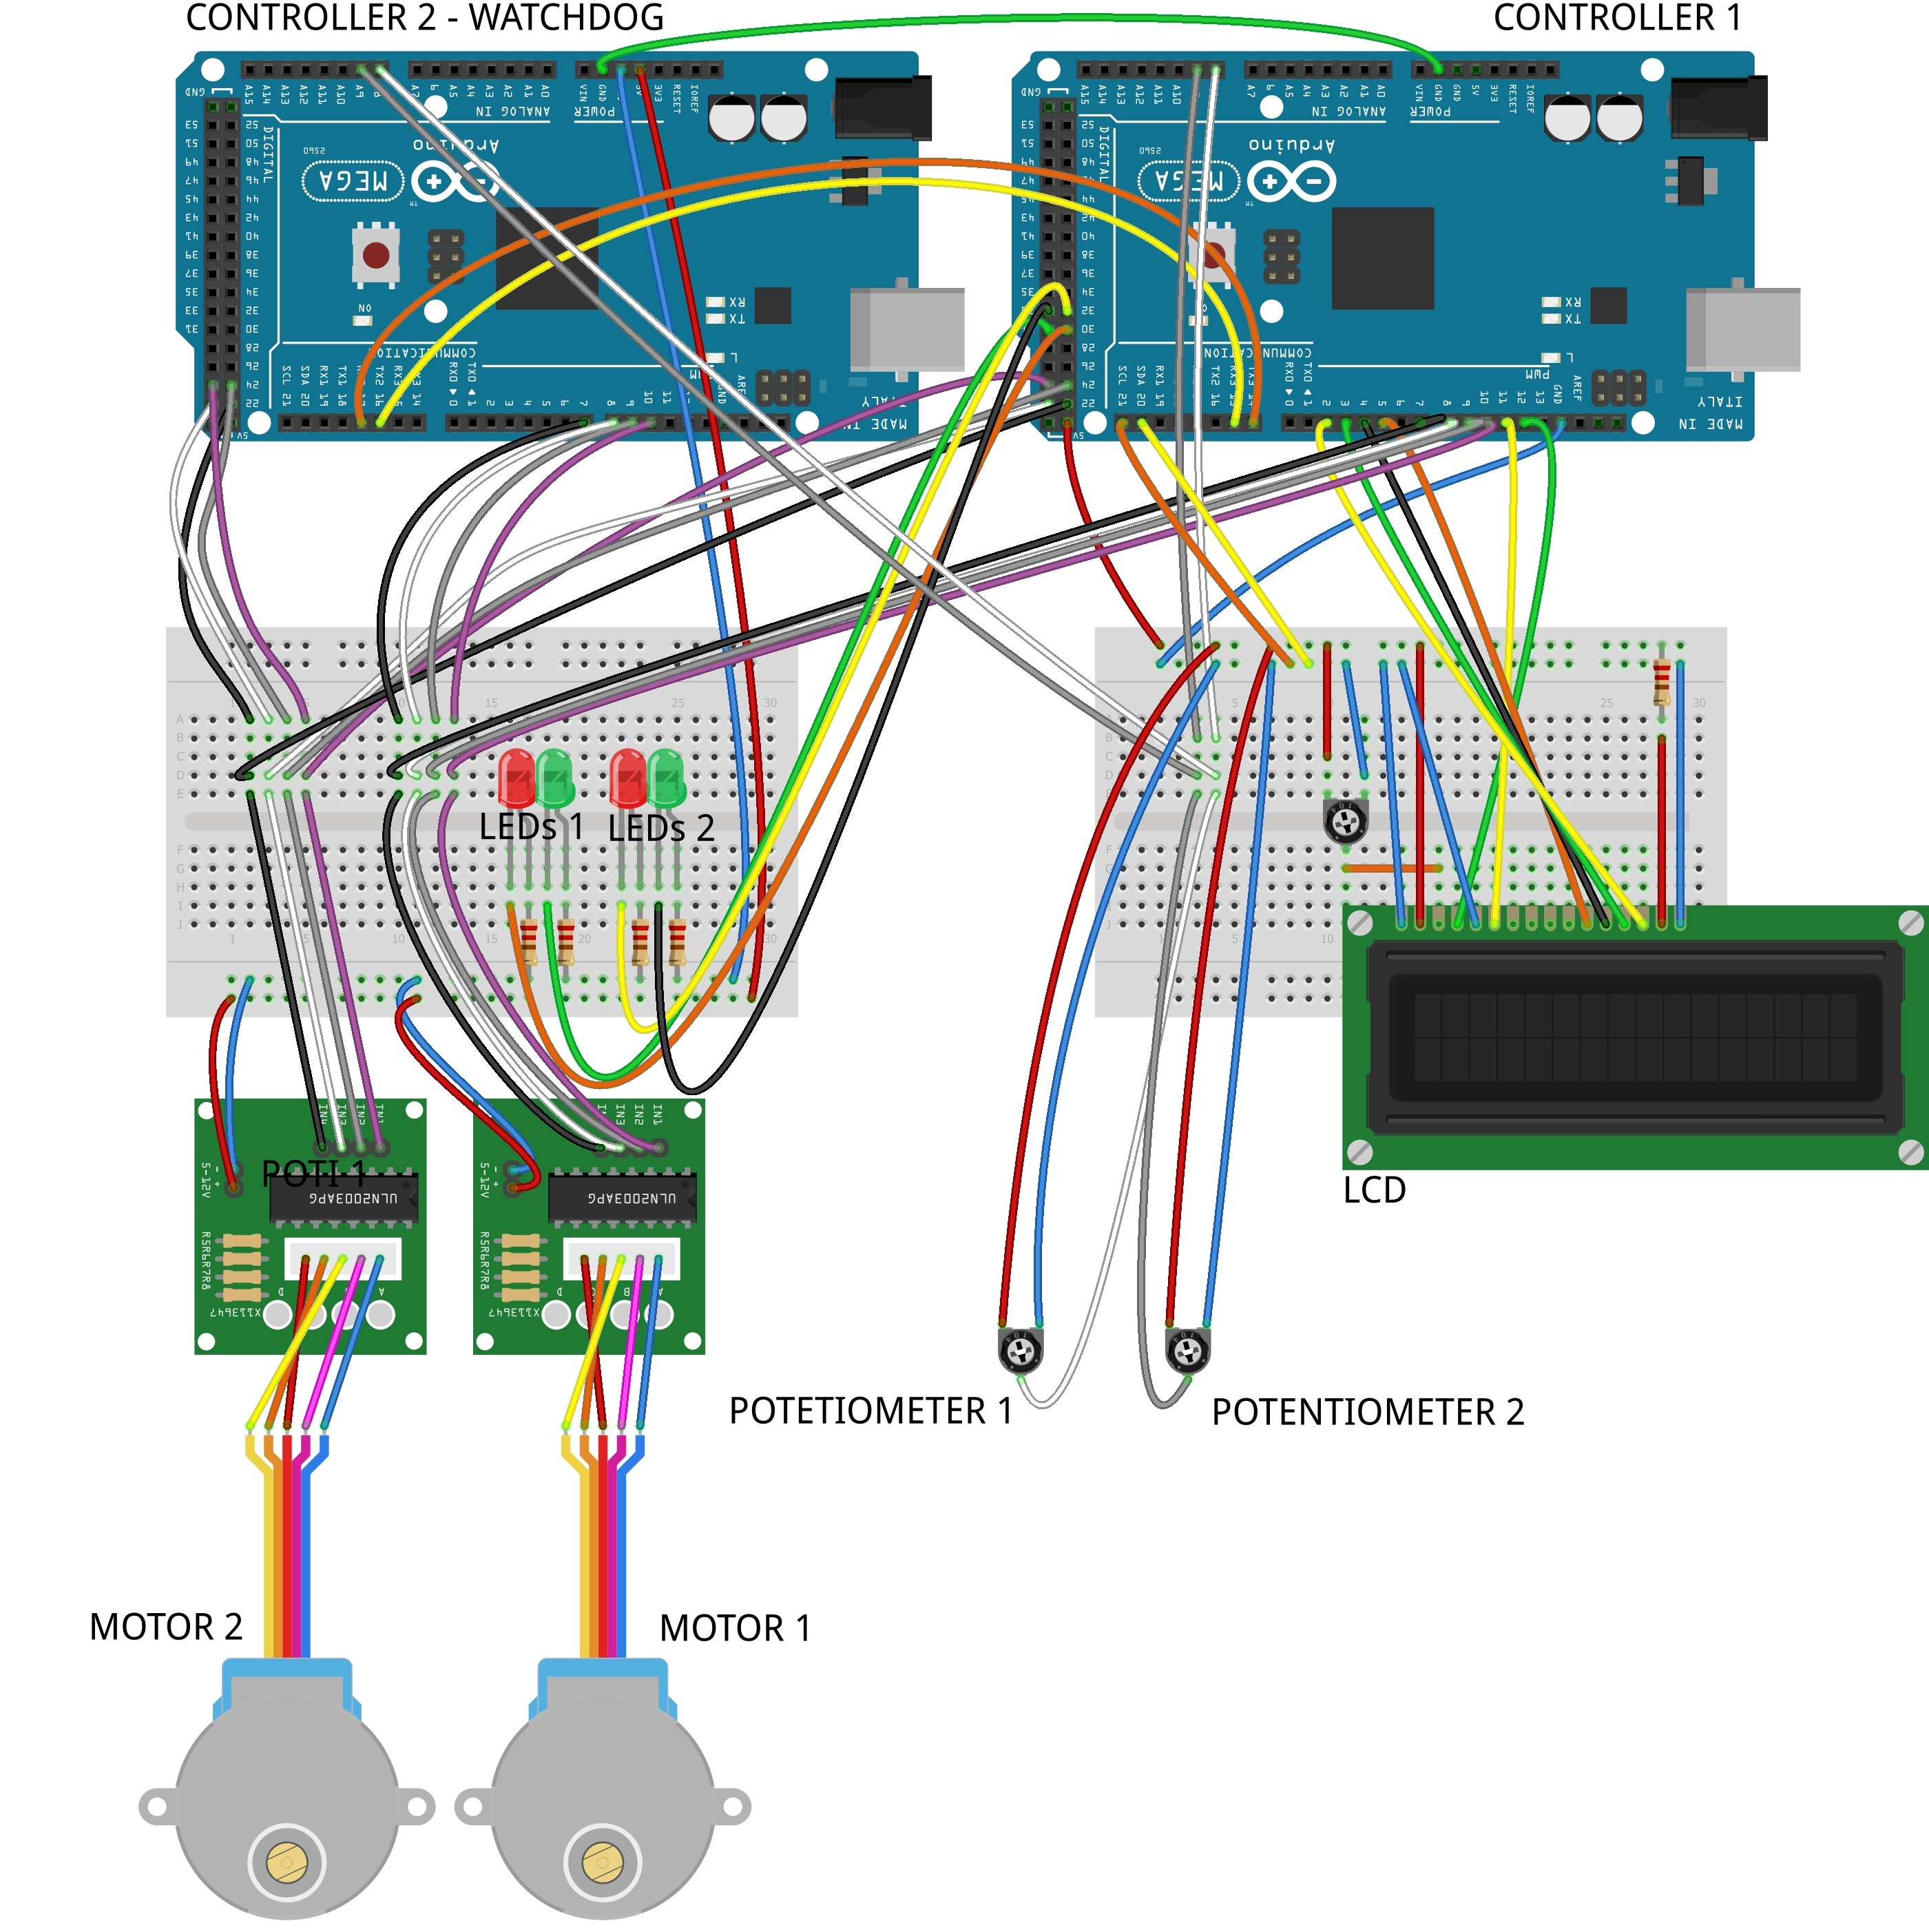
\includegraphics[width=0.7\textwidth]{figures/circuit.jpg}
    \caption{Circuit schematic}
     \label{fig:circuit_schematic}
\end{figure}

As explained in \autoref{sec:preliminary_analysis}, verification of the angle is necessary since the stepper motor alone does not return adequate feedback about its position.  Here, potentiometers are used to detect the angular position of the solar panel and verify if the assigned angle is reached. To verify the functionality of the system sufficiently, a pair of potentiometers receives the motor's rotation through the connected axis, compare \autoref{fig:mech_design}, and votes on the status of the system. The experimental setup only uses two potentiometers instead of the needed four to also receive feedback on the second stepper motor's position. The complete setup is considered to be analog to the first stepper motor's configuration and executed from the experimental design but implemented into the software architecture. The potentiometers sit close to each other and are powered, likewise to the motors, through the Arduino board.

Further, the system possesses two buttons represented by two cables that connect to pin 20 and 21 of the Arduino master board. The former is forcing the system into its safe mode - meaning the solar panel is rotated to a predefined safe angle. The latter is initiating a reset frequency, after which normal operation can be continued.

\subsection{Mechanical design}
\autoref{fig:mech_design} shows the mechanical set-up of the solar panel drive mechanism. On the left side, the stepper motors are attached to the wooden stand representing the mounting structure. Opposite, the redundant potentiometer pair is embedded into the stand and connected through a wooden axis to stepper motor 1. The mock-up solar panel is fixed to the wooden axis. Thus, the rotation of the stepper motor is conveyed to the potentiometers, while the solar panel moves according to the user's input. Theoretically, once the second stepper motor takes over, it must be able to drive the solar panel. Due to the mechanical complexity of this configuration, it is not included in the experimental design. That structure is out of the scope of this project, since the stepper motors are not capable of forcing each other's movement in case of failure.


\begin{figure}[H]
    \centering
    \begin{subfigure}[b]{0.49\textwidth}
       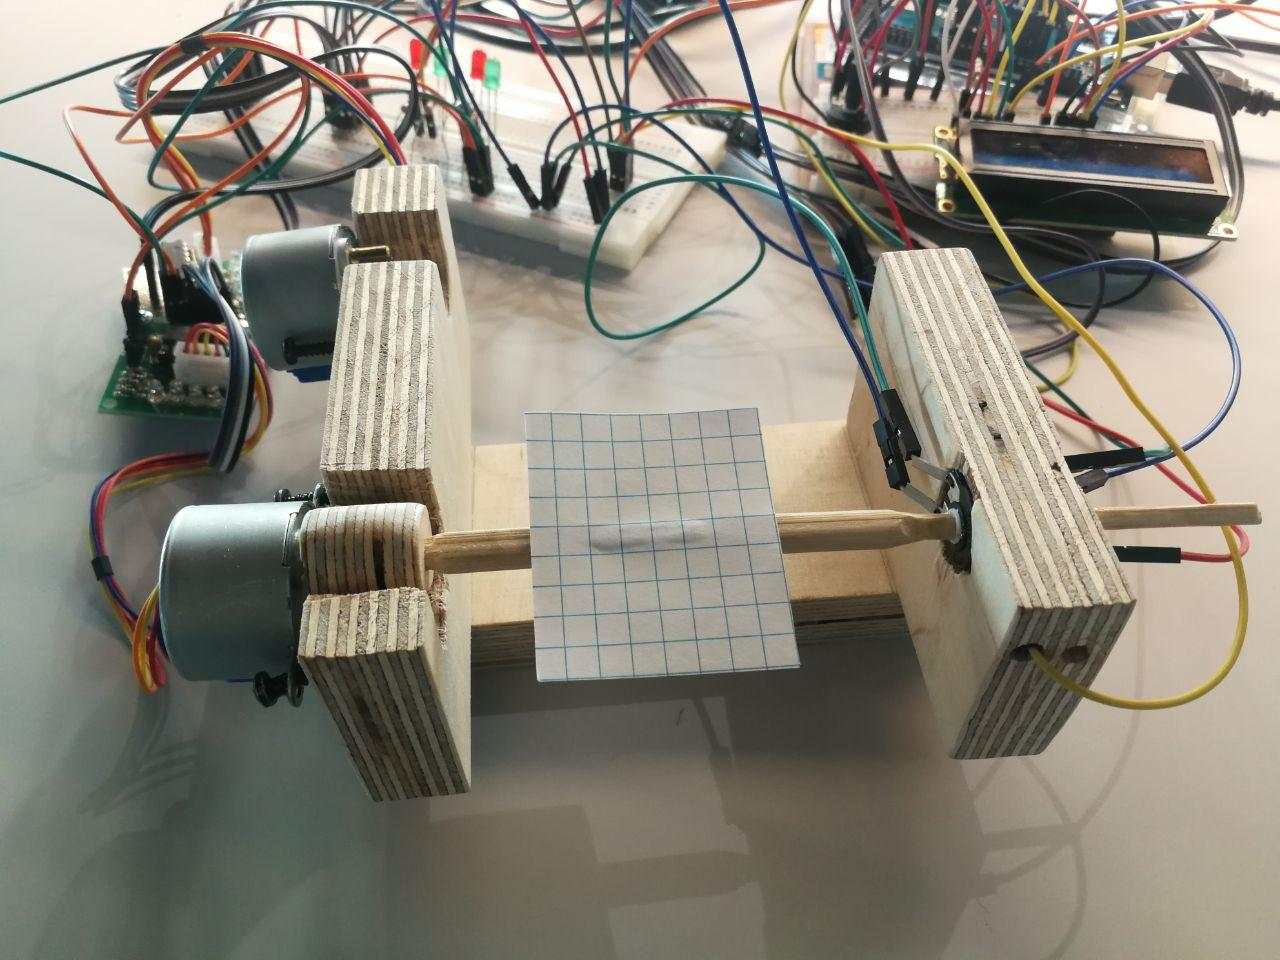
\includegraphics[width=\textwidth]{figures/mech01.jpg}
    \end{subfigure}
    \begin{subfigure}[b]{0.49\textwidth}
       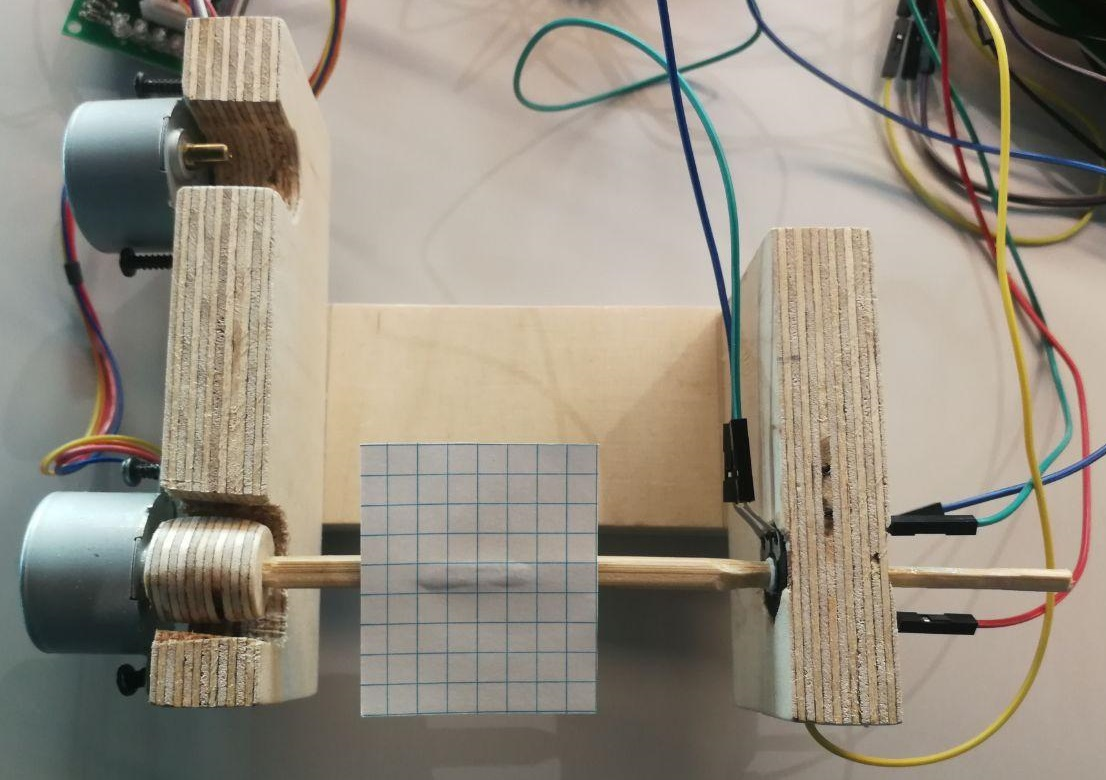
\includegraphics[width=\textwidth]{figures/mech02.jpg}
    \end{subfigure}
    \caption{Solar panel mounting structure}
    \label{fig:mech_design}
\end{figure}{}




\pagebreak
\section{Fault detection, isolation and recovery}
\label{sec:fdir}

Following the subsystem design and software architecture, this chapter analyses which faults can occur during normal operation. Related with the preliminary failure study in \autoref{sec:preliminary_analysis}, this analysis subdivides the faults into the actuators, sensors and microcontrollers - stepper motors, potentiometers and Arduinos, respectively.

This chapter follows the fault detection, isolation and recovery (FDIR) methodology: the system must detect the faults and isolate them, to avoid mission failure. Then, the controllers perform the recovery process according to 4 FDIR levels (L0 to L3). The fault analysis follows the schematic in \autoref{fig:fault_tree}. This methodology can be found in the Arduinos' source code (in appendices \ref{appendix:master} and \ref{appendix:slave}).


\begin{figure}[H]
    \centering
    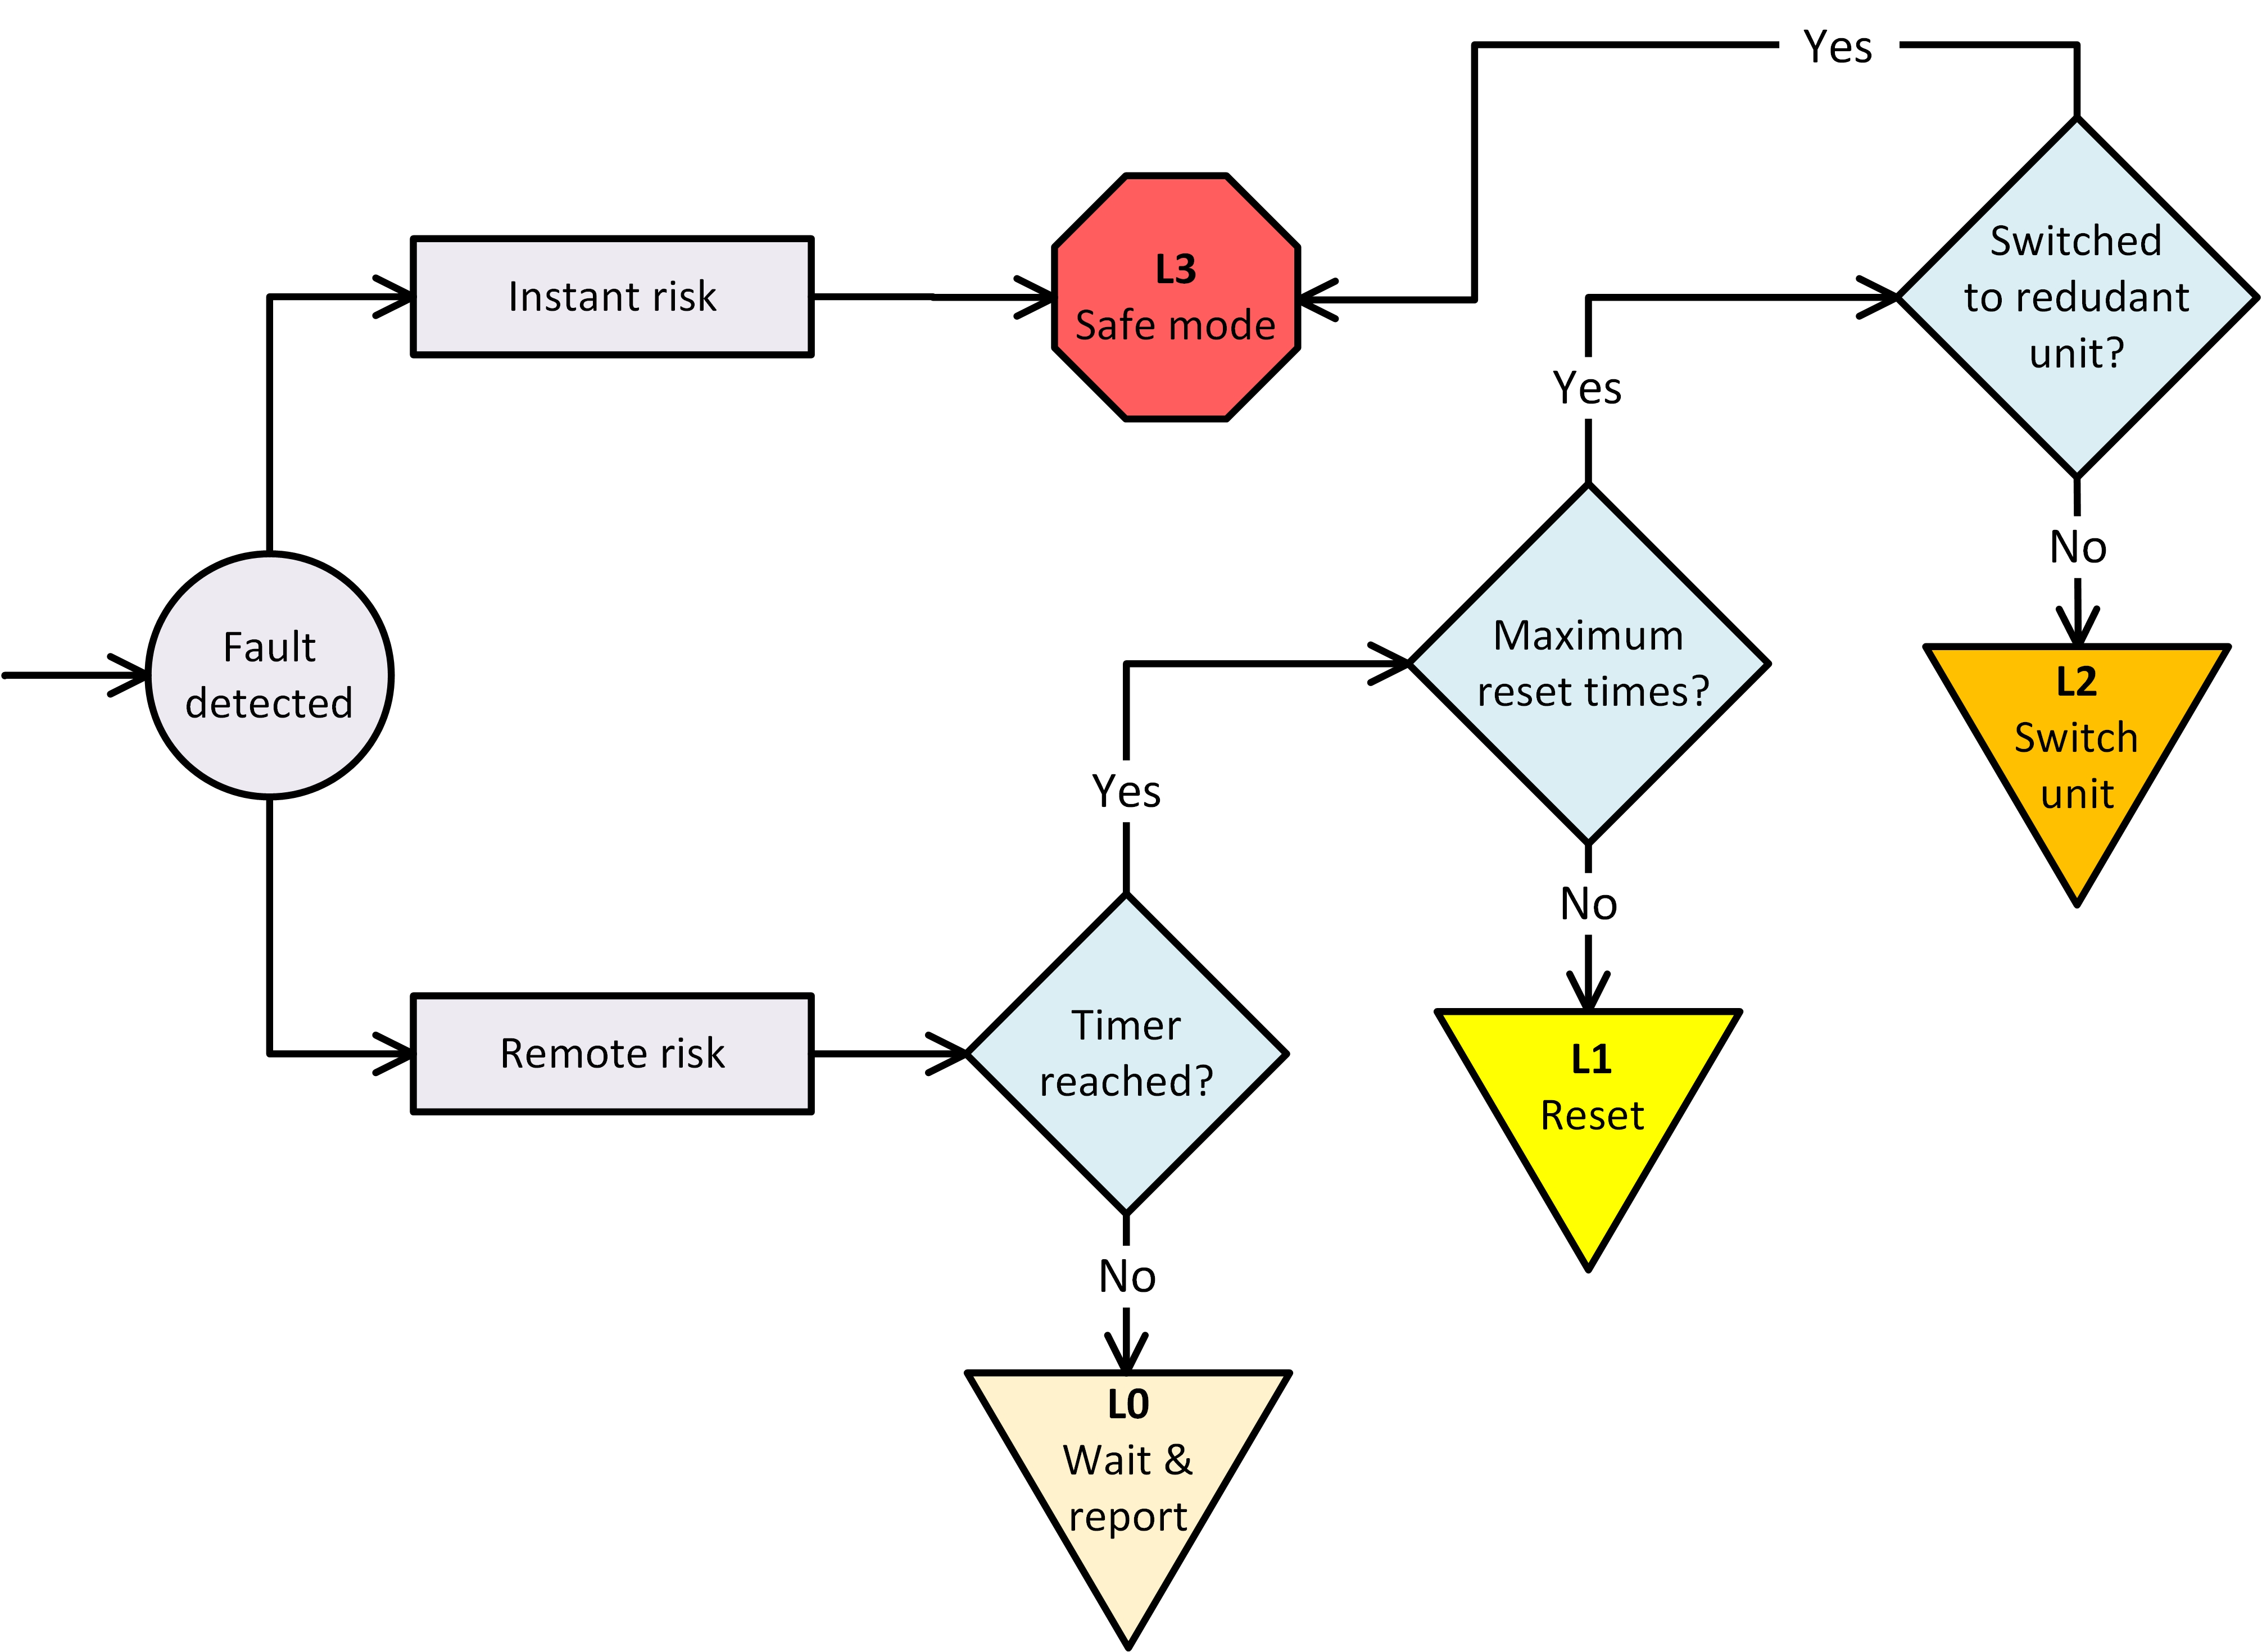
\includegraphics[width=0.8\textwidth]{figures/fdir.jpg}
    \caption{General fault recovery tree (for actuators, sensors and controllers). The timer cycle period and maximum reset times numbers are defined in \autoref{sec:fdir}.}
    \label{fig:fault_tree}
\end{figure}

Following the logic in \autoref{fig:fault_tree}, ideally, the resets (and the safe mode) can be manually or automatically triggered. Given that the communication between the computer, Arduinos and peripherals is in the order of milliseconds, the time it takes for a reset to take place is set to 5 seconds. This schematic applies entirely for the actuators and microcontrollers, while the sensors -- potentiometers -- work simultaneously and, therefore faults can only be reported (up to L0). 

The maximum reset times for the master microcontroller is one, i.e., if the slave microcontroller attempts to reset the master two times \textbf{consecutively}, the slave board takes control of the subsystem. Given the mechanical design of the mock-up, the secondary stepper motor rotates only when the sensors and primary motor disagree altogether. This option is not the ideal FDIR approach: if both stepper motors could turn the shaft (and consequently the solar panel), the controllers could implement a TBD maximum number of reset times of the primary stepper motor, after which the redundant unit would be switched on. Finally, the experimental design in \autoref{sec:experimental} cannot detect faults in the redundant units -- both the stepper motor and Arduino. Thus, the safe mode can only be manually triggered (experimentally). The ideal design would require additional units (sensors, mainly) and a more complex mechanical structure.



Faults are coded as \textit{xy}: \textit{"x"} represents the faulty component and \textit{"y"} the error number.

% communication not established, although controller 1 still working
%  -- both sending command to stepper
 
 
\subsection{Stepper motor}

\begin{table}[H]
    \centering
    \begin{tabular}{c|c|c}
        Component & ID & Description \\ \hline \hline
        \multirow{3}{*}{
            \begin{tabular}{c} Stepper\\Motor \end{tabular}}& 11 & Drift/block \\ \cline{2-3}
            & 12 & No power/No response\\ \cline{2-3}
            & 13 & No feedback \\ \hline
    \end{tabular}
    \caption{Stepper motor faults}
    \label{tab:stepper_faults}
\end{table}


\paragraph{Drift/block\\}

This fault occurs when the stepper motor rotates more (or less) than what it needs, to match the user input. It is most likely to occur with a higher number of solar panel movements, as mechanical imperfections, fluctuations in power input and low torque may affect the rotation.

Sensors, such as potentiometers, can be used to \textbf{detect} this fault. The feedback from one (or more) potentiometers, along with the motor's step information, with an appropriate voting system, provides the microcontrollers sufficient data to acknowledge the stepper's approximate true position. Thus, when the stepper drifts more than a predefined margin (or even when it blocks), the voting system can choose which angle is the actual true position. Following the tree in \autoref{fig:fault_tree}, the microcontroller resets the stepper's position. This method consists of a triple modular passive redundancy since it uses three inputs and (software) voter.

Theoretically, after a TBD number of reset times, the redundant unit should be activated (hot standby). However, due to the mock-up physical limitations, if the voter cannot determine the panel's true position, the redundant unit is activated (L2), since it is assumed that the initial stepper cannot operate the panel properly.

\textbf{Isolation} consists of detecting if both sensors acknowledge the drift/block. If the sensors are deemed to be operating correctly, then the fault 11 is correctly isolated. Otherwise, the controllers must perform a deeper sensor analysis.

In this case, if the stepper drifts and both potentiometers agree on this, L0 is skipped: the system resets the stepper's angle electronically. If an imminent crash may occur, safe mode can be manually activated. Once again, if the operator detects that the secondary stepper motor is incorrectly operating, safe-mode can also be activated (L3).




\paragraph{No power/No response\\}

If the subsystem fails to provide energy to the stepper, the motor cannot move. This fault is a sub-type of fault 11 since the stepper's response will be experimentally equal. In case that the motor does not react to the user's input, the panel's sensors (potentiometers) can detect this faulty operation. Given that the Arduino computes the stepper motor's instant step electronically, the microcontroller can assume an instant step increase/decrease with time even if the stepper blocks. Therefore, the software can only rely on the sensors to detect and isolate faults 11 and 12.

Thus, the FDIR approach, in this case, is similar to fault 11.



\paragraph{No feedback\\}

 












\subsection{Potentiometer}
















\begin{table}[H]
    \centering
    \begin{tabular}{c|c|c}
        Component & ID & Description \\ \hline \hline
        \multirow{4}{*}{Potentiometer} & 21 & No feedback \\ \cline{2-3}
            & 22 & Potentiometers disagree with each other\\ \cline{2-3}
            & 23 & Potentiometers disagree with stepper motor \\ \cline{2-3}
            & 24 & Feedback is not constant \\\hline
    \end{tabular}
    \caption{Potentiometers faults}
    \label{tab:pot_faults}
\end{table}

potentiometers are already protected to not go out of bounds from the start;

\subsection{Microcontroller}

\begin{table}[H]
    \centering
    \begin{tabular}{c|c|c}
        Component & ID & Description \\ \hline \hline
        \multirow{3}{*}{Microcontroller} & 31 & No power/No connection \\ \cline{2-3}
            & 32 & No communication between Arduinos\\ \cline{2-3}
            & 33 & No response to input \\ \hline
    \end{tabular}
    \caption{Microcontrollers faults}
    \label{tab:microcontroller_faults}
\end{table}
\pagebreak
\section{Software architecture}
Following the hardware design and FDIR, this section elaborates on the system's software architecture. Appendix \ref{appendix:master} and \ref{appendix:slave} show the code of the master and slave Arduino respectively. The Arduino software IDE is an application that conveniently allows one to write and alter the code and upload it directly to the boards, which are then operated from the Arduino IDE serial monitor.

\subsection{General setup}
After including the libraries needed for the operation of the stepper motor, LCD, and various Arduino functions, the used constants, variables, flags, and actuator and sensor pins are initialized. Serial communication is established and allows for more detailed feedback regarding the systems' status. 

The user commands the solar panel drive mechanism through the serial monitor. The system asks to receive an angle within a certain range. If the user input is not located within this range, the angle is set to the lowest and highest possible angle depending on the input given. The system informs the user about the input provided and how the system is reacting to it, compare function \textit{$check_input()$} in appendix \ref{appendix:master}. Before the motor rotates the direction in which the rotation shall be performed is checked. This is necessary since the potentiometers cannot support the continuous rotation of the stepper motor and constrain the motor's movement to a range of 270\degree \pm 10\degree. While the motors are in standby each of the green LEDs is on. Rotates a motor the green and red LED of the respective motor signals its activity. Is a motor considered to be not operational, e.g. a reset of the motor angle has failed, the red LED is switched on. 




After the stepper motor's rotation of the solar panel, the stepper motor's and the potentiometers' feedbacks are read. 



%init_value 
in order to validate the stepper motor's position 
use estimated potentiometer functions further explained in \autoref{sec:experimental}. 
retrieve the feedback on the potentiometers output 
angle obtained is compared
If both potentiometers agree on the range in which the angle is located the average of both potentiometers is used to verify the stepper motor's position
this way, at least one potentiometer has to agree with the stepper motor in order to continue the operation.
In case both potentiometers disagree with the user input's angle after the motor has moved to its assigned position a command is sent to reset the motors position to the potentiometers feedback.
Further, if both potentiometers agree on the current angle of the solar panel but disagree with the stepper motor's feedback it is assumed, that the motor has drifted. The system is then performing a reset of the stepper motor, meaning a reset of the motor's angle to the potentiometer's value. The motor reset can also be performed manualy by setting pin 21 to HIGH. If for any reason, such as no matching potentiometer value, a stepper motor reset cannot be performed, the system switches to the redundant unit and stepper motor 2 is now in operation.

Additionally, the system possesses a safe mode, which functions likewise to the motor reset as an interrupt. Here, if pin 20 is triggered and set to HIGH the active motor moves into the defined minimum angle and the system is forced into standby.



include libaries
initialize variables, etc.

operating the actuators and sensors

panel driving
verification
feedback (visual)
fault detection

interrupts: safe mode, reset



\subsection{Master vs slave board architecture}
The microcontroller are operating in hot standby, while the second board functions as a watchdog.

The master Arduino transmits every second to the slave Arduino, in order to reset the watchdog's timer.






add graphics




generally, before switching components send reset command, if not effective switch component


motor does not give direct feed back and no encoder 
following an potentiometer is used to keep track and give feedback


redefine zero angle of stepper with poti position


tolerance  at 0 for serial input
7 for 

reset button, cable used:


to do:


activate second motor, check if working:    did that

integrate second board, establish communication: check

integrate second poti -> big range until glued
compare poti results  :
are they within the same margin of values (approx. 120)
as long as one poti agrees with stepper keep stepper running
if both disagree switch to stepper two

decide if motor 1 should still be working

reset button. done
alternative if both potis dont aggree, mission over, sucker.
%%%%%%%%%%%%%%%%%%%%%%%%%%%%%%%%%%%%%%%%%%%%

reset of motor one if out of range

reset options


%%%%%%%%%%%%%%%%%%%%%%%%%%%%%%%%%%%%%%%%%%%%

integrate watchdog takeover
master updating status: hey I'm fine
slave: cool, dude
if master not sending * ..... *
slave: dude, think you're dead, taking over now
slave receiving and sending commands



%%%%%%%%%%%%%%%%%%%%%%%%%%%%%%%%%%%%%%%%%%%


led feedback: done
red not working
green operational, on stand by
green plus 



%not happening: attach third poti to second motor with plastic, use heat



poti within range of 100 950
define possible usable angles as user input




don't forget to reference source code
\ref{appendix:master}
\ref{appendix:slave}
\pagebreak
\section{Experimental implementation}
\label{sec:experimental}



\begin{figure}[H]
    \centering
    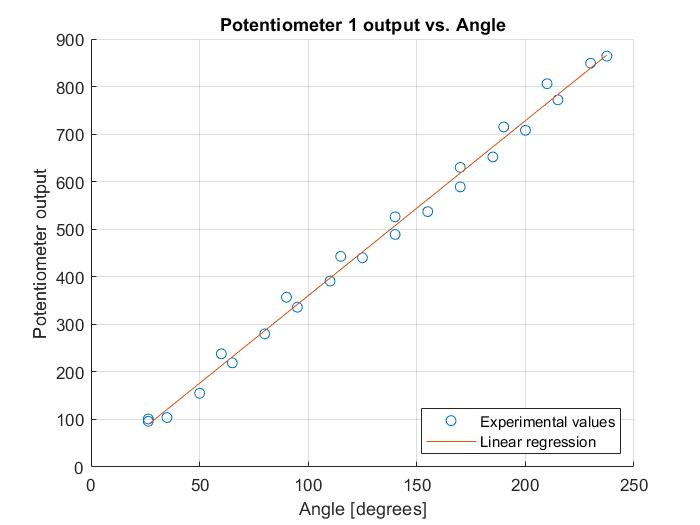
\includegraphics[width=0.7\textwidth]{figures/pot1.jpg}
    \caption{Relation between angle and potentiometer 1 output}
    \label{fig:pot1}
\end{figure}

\begin{align*}
    \begin{cases}
        y = 3.6806\,x  - 7.8262 \\
        R^2 = 0.9966
    \end{cases}
\end{align*}

\begin{figure}[H]
    \centering
    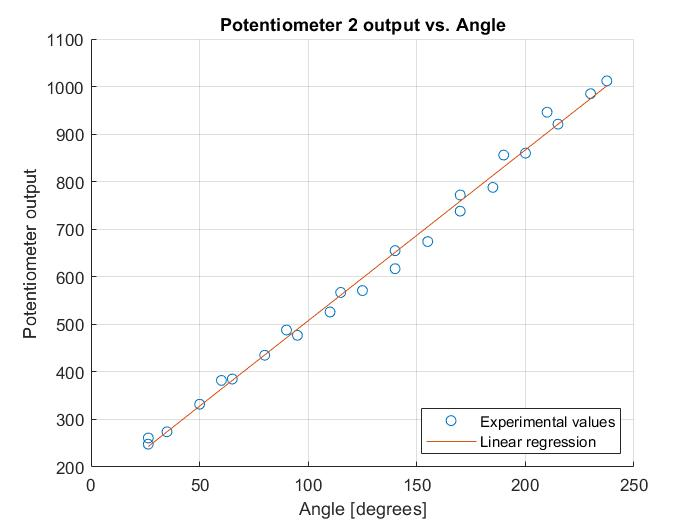
\includegraphics[width=0.7\textwidth]{figures/pot2.jpg}
    \caption{Relation between angle and potentiometer 2 output}
    \label{fig:pot2}
\end{figure}

\begin{align*}
    \begin{cases}
        y = 3.5921\,x + 148.3947 \\
        R^2 = 0.9969 
    \end{cases}
\end{align*}



\begin{figure}[H]
    \centering
   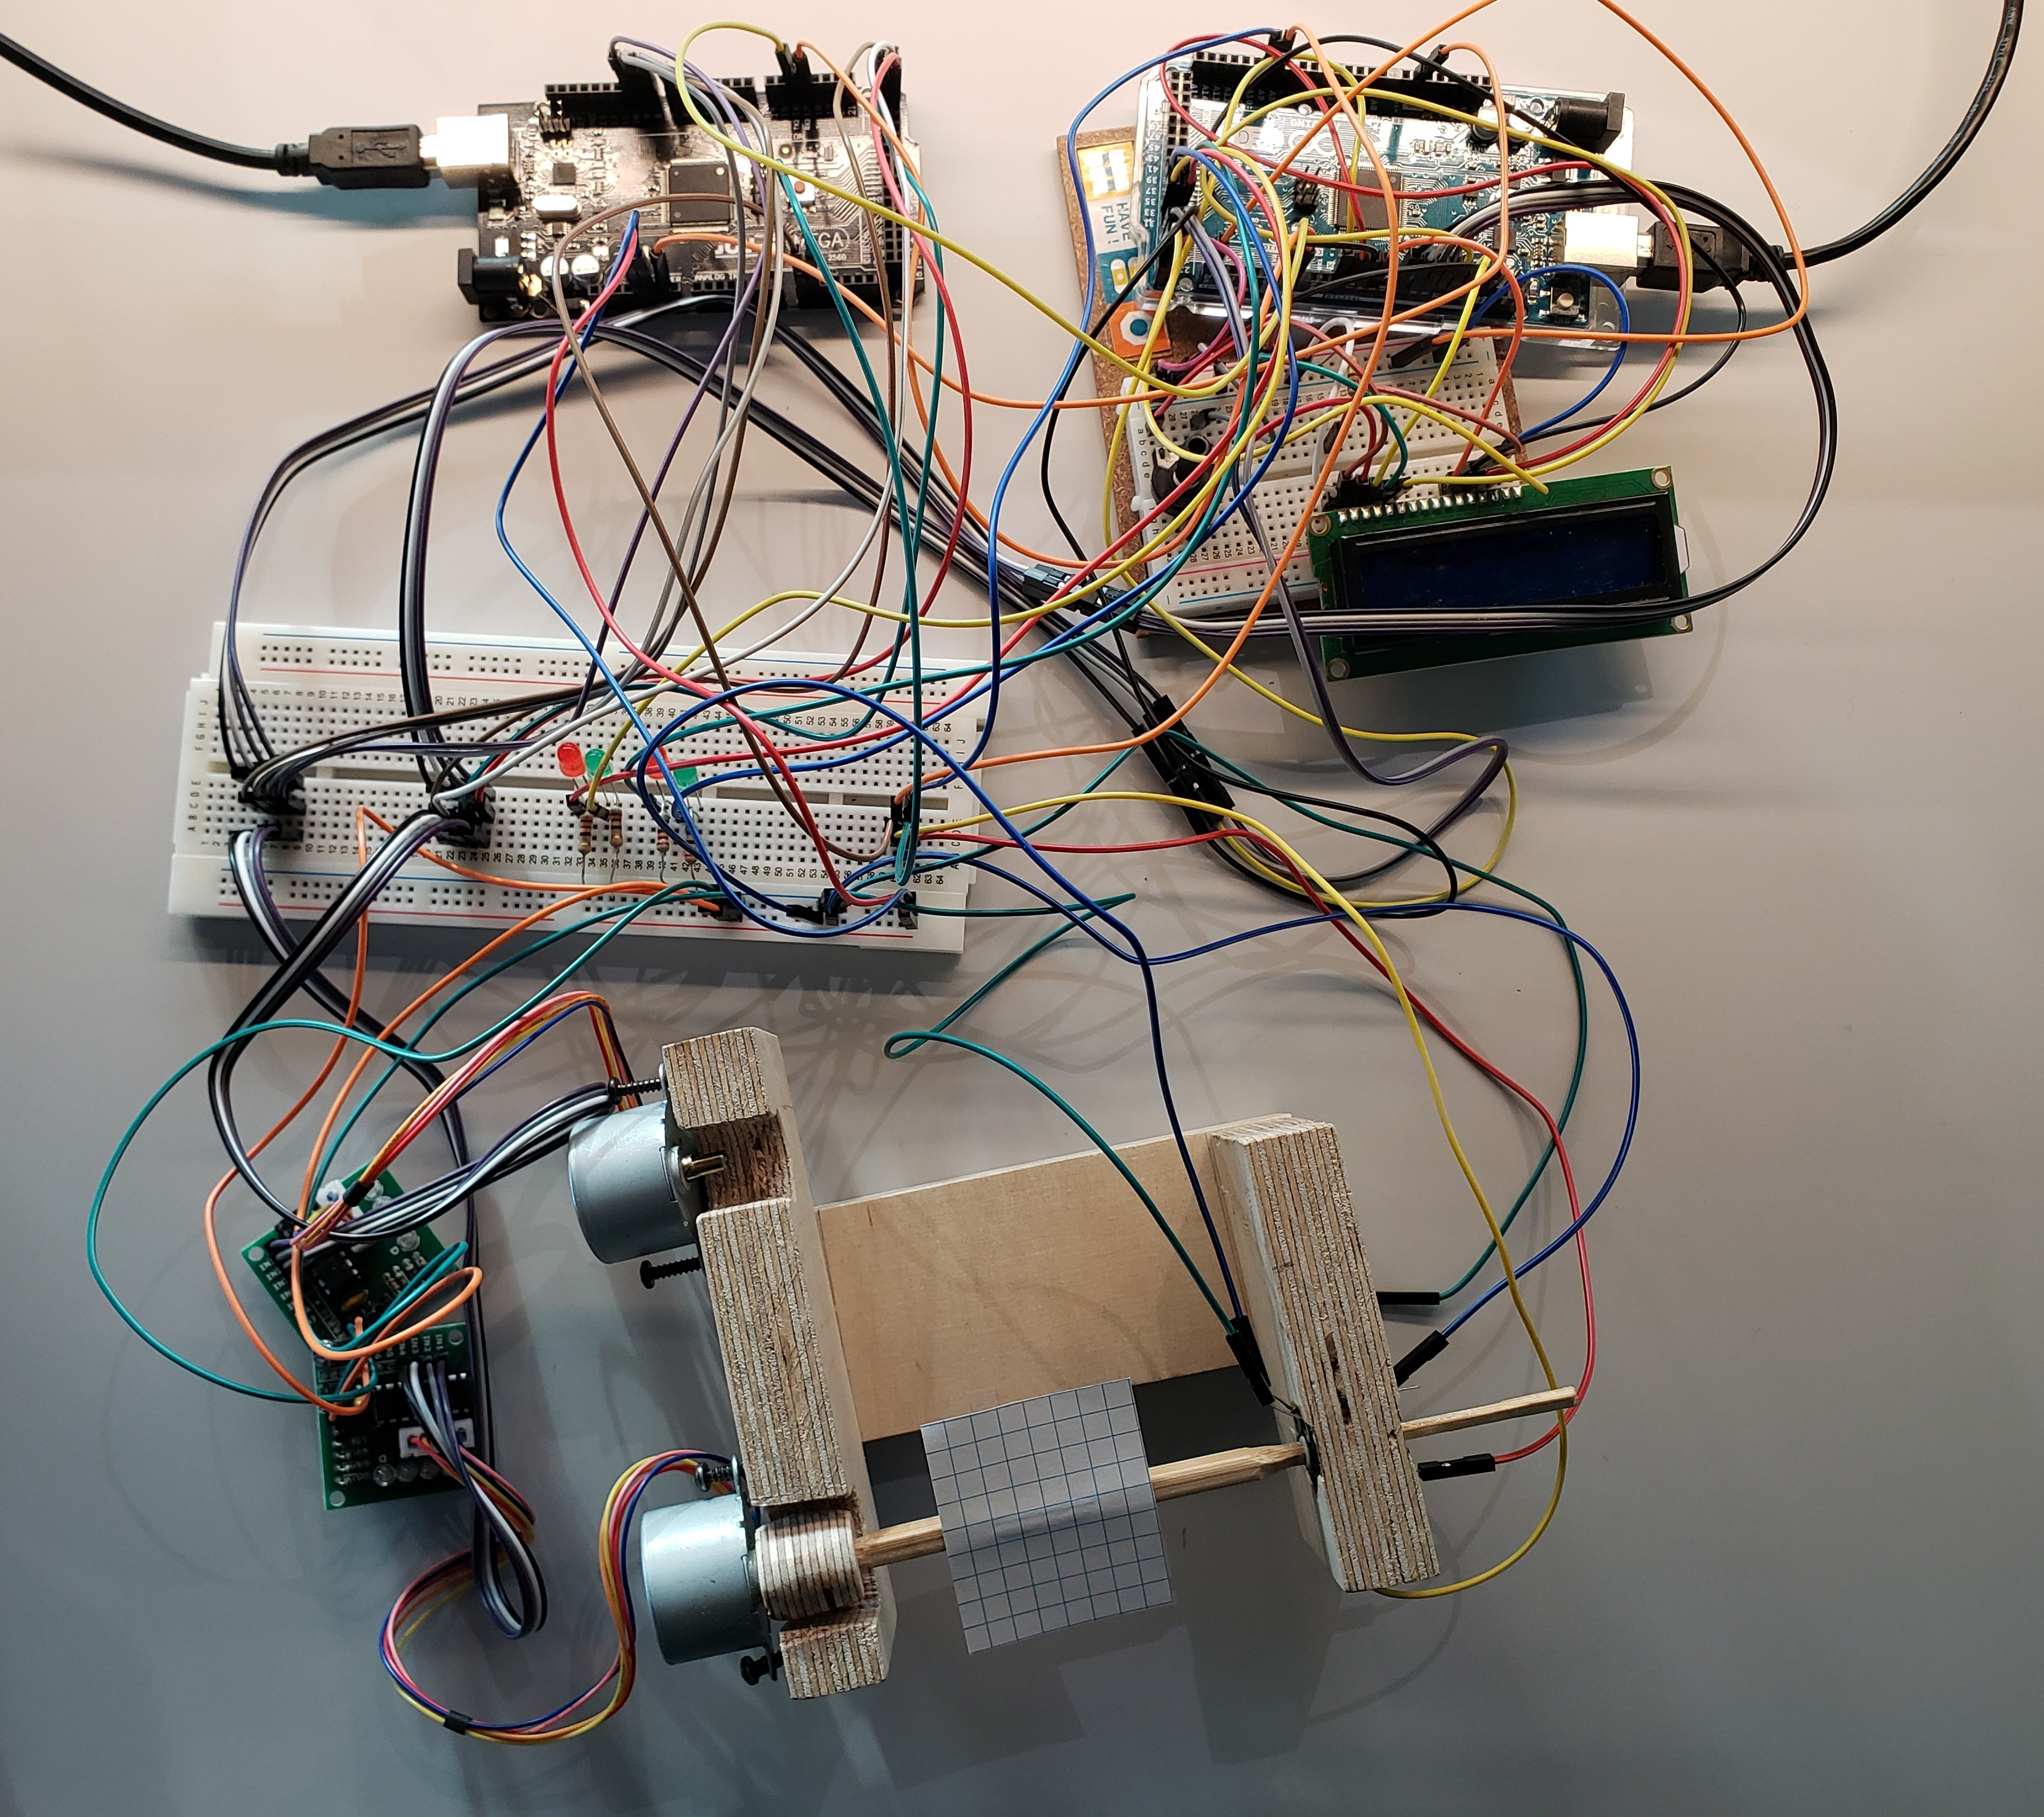
\includegraphics[width=\textwidth]{figures/circuit_pic.jpg}
    \caption{Circuit schematic}
     \label{fig:implented_design}
\end{figure}



add specific angle range that can be used
\pagebreak
\section{Final remarks and recommendations}

also include what and why is not perfect
explain how it could be better in a larger application/system

 -- if only communication between the boards is interrupted, both send signals to the motors, etc. system fails


hand in video of explaining the project




\pagebreak



\nocite{lecture_slides}



\begin{appendices}
\appendix
\section{- Source code (Arduino)}
\subsection{\texttt{stepper.ino} - Master board}
\label{appendix:master}
\lstinputlisting[language=c++, basicstyle=\scriptsize\ttfamily]{source_code/stepper.ino}

\pagebreak
\subsection{\texttt{stepper\_slave.ino} - Slave board}
\label{appendix:slave}
\lstinputlisting[language=c++, basicstyle=\scriptsize\ttfamily]{source_code/stepper_slave.ino}

\end{appendices}

\pagebreak
\bibliographystyle{acm}
\bibliography{mybib}

\end{document}